\documentclass{proposal}
\graphicspath{{./fig/}}

\title{Theory of Discrete Fourier Transform and Cross-correlation function} % Title
\author{Kurama Okubo} % Author name
\date{\today} % Date for the report
\begin{document}
\maketitle

\section{Introduction}
In this note, we describe the definition of Fourier transform, Inverse Fourier transform, Discrete Fourier transform (DFT), Inverse Discrete Fourier transform (IDFT) and Cross-correlation function for time series analysis.
 
\section{Definition}

Let $f(t)$ be a time series (\textit{e.g.} acceleration [m/s$^2$], velocity [m/s], displacement [m]). The unit of $t$ is time [s]. 
\begin{description}
\item[Euler's formula]
\begin{equation}
e^{i\theta} = \cos{\theta} + i\sin{\theta},
\end{equation}
where $i$ is imaginary unit.
\item[Fourier Transform]
\begin{equation}
F(\omega) = \int_{-\infty}^{+\infty} f(t) e^{-i\omega t} dt = \mathcal{F}[f(t)],
\end{equation}
where $\omega$ is frequency [Hz]. $\mathcal{F}$ indicates the Fourier transform operation.
\item[Inverse Fourier Transform]
\begin{equation}
f(t) = \frac{1}{2\pi} \int_{-\infty}^{+\infty} F(\omega) e^{i\omega t} d\omega = \mathcal{F}^{-1}[F(\omega)].
\end{equation}
Thus
\begin{equation}
\mathcal{F}^{-1}[\mathcal{F}[f(t)]] = f(t).
\end{equation}

\item[Cross-correlation function] ~
\\Let $u_1(t)$ and $u_2(t)$ be time series.

\begin{equation}
\psi_{12}(\tau) =  \int_{-\infty}^{+\infty} u_1(t)u_2(t+\tau) dt.
\end{equation}

When $u_1(t)$ and $u_2(t)$ are finite duration time series ($t_1 \leq t \leq t_2$), the cross-correlation function is defined as
\begin{equation}
\psi_{12}(\tau) =  \int_{t_1}^{t_2} u_1(t)u_2(t+\tau) dt,
\end{equation}

where
\begin{equation}
-(t_2 - t_1) \leq \tau \leq (t_2 - t_1). 
\end{equation}

\item[Cross spectrum] ~
\begin{equation}
\Psi_{12}(\omega) = U_1^*(\omega)U_2(\omega),
\end{equation}
where $U_1^*$ is complex conjugate of $U_1(\omega)$. It is noteworthy that \textcolor{red}{we assume the periodicity of finite duration time series $[t_1, t_2]$} to regard it as  infinite duration time series. Thus $-\infty < \omega < \infty$.
 
Then
\begin{equation}
\psi_{12}(\tau) = \mathcal{F}^{-1}[\Psi_{12}(\omega)].
\end{equation}


\begin{figure}
\center
\noindent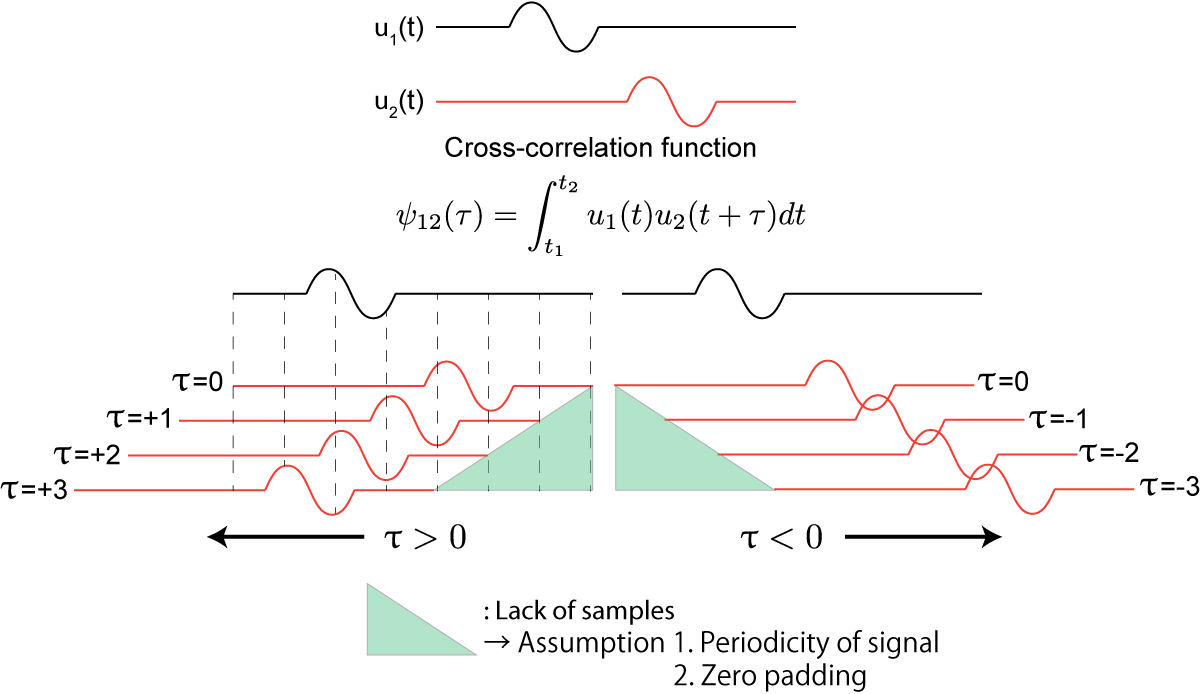
\includegraphics[width=\textwidth]{crosscorrelation.png}
\caption{Schematic of Cross-correlation function.}
\label{fig:xcorr}
\end{figure}


\item[Discrete Fourier Transform (DFT)] ~ 
\\Let $u[n]$ be a discrete time series. $n=0,1,2, \cdots, N-1$, where $N$ is data length. Then $t = n\times dt$.  
\begin{equation}
U[k] = \sum_{m=0}^{N-1}u[m]e^{-\dfrac{i2\pi km}{N}}. \quad k = 0,1,2, \cdots, N-1
\end{equation}

\item[Inverse Discrete Fourier Transform(IDFT)]
\begin{equation}
u[n] = \dfrac{1}{N} \sum_{l=0}^{N-1} U[l] e^{\dfrac{i2\pi ln}{N}}. \quad n = 0,1,2, \cdots, N-1
\end{equation}
Then
\begin{equation}
u[n] = IDFT[DFT[u[n]]].
\end{equation}

\item[Discrete Cross-correlation function]
\begin{equation}
\psi_{12}[n] = \sum_{k=0}^{N-1}u_1[k]u_2[k+n]. \quad n = 0, \pm1, \pm2, \cdot, \pm(N-1)
\end{equation}
Thus the size of $\psi_{12}[n]$ is $2N-1$. $t = n\times dt$.
For the Discrete Cross spectrum, we can also define the Discrete Cross-correlation function as following:
\begin{equation}
\psi_{12}[n] = \begin{cases}
\sum_{k=0}^{N-1}u_1[k]u_2[k+n] & n = 0,1,2, \cdots, N-1\\
\sum_{k=0}^{N-1}u_1[k-n]u_2[k]  & n = -1,-2, \cdots, -(N-1)
\end{cases}.
\end{equation}

\begin{itembox}[l]{Note}
For negative $n$, shifting $u_2$ towards right-hand side is identical with shifting $u_1$ towards left-hand side (See Figure \ref{fig:xcorr}).
\end{itembox}

\item[Discrete Cross spectrum]
\begin{eqnarray}
\Psi_{12}^{+}[k] &=& U_1^*[k]U_2[k] \quad (k \geq 0)\\
\Psi_{12}^{-}[-k] &=& U_1[-k]U_2^*[-k] \quad (k < 0).
\end{eqnarray}
where $-(N-1) \leq k \leq (N-1)$.
\begin{itembox}[l]{Note}
Since the definition of DFT allows the index to be only positive, we have to consider the conditions $k\geq0$ or $k<0$.
\end{itembox}

Then
\begin{equation}
\psi_{12}[n] = \begin{cases}
IDFT[\Psi_{12}^{+}[n]] & n = 0,1,2, \cdots, N-1\\
IDFT[\Psi_{12}^{-}[-n]] & n = -1,-2, \cdots, -(N-1)\
\end{cases}.
\end{equation}

\item[Fast Fourier Transform (FFT)] ~
\\FFT is the algorithm to obtain the components of DFT effectively by using periodicity to reduce the calculation.

\end{description}


\section{Derivation}
\begin{lemma}
\begin{equation}
\mathcal{F}^{-1}[\mathcal{F}[f(t)]] = f(t).
\end{equation}
\end{lemma}

\begin{proof}
\begin{eqnarray}
\mathcal{F}^{-1}[\mathcal{F}[f(t)]]  &=& \frac{1}{2\pi} \int_{-\infty}^{+\infty} \left[\int_{-\infty}^{+\infty}  f(t') e^{-i\omega t'} dt'\right] e^{i\omega t} d\omega \\
&=& \int_{-\infty}^{+\infty}  f(t') \left[ \frac{1}{2\pi} \int_{-\infty}^{+\infty} e^{-i\omega (t' - t)} d\omega \right] dt'.
  \label{eq:ft1}
\end{eqnarray}
Since
\begin{eqnarray}
 \int_{-\infty}^{+\infty}  e^{-i\omega (t' - t)} d\omega &=& \lim_{a \to \infty} \left(\int_0^{a} - \int_0^{-a} \right)  e^{-i\omega (t' - t)} d\omega \\
 &=& \lim_{a \to \infty}  \dfrac{2\pi \sin{a(t'-t)}}{\pi(t'-t)} \\
 &=& 2\pi \delta(t'-t),
\end{eqnarray}
where $\delta(t'-t)$ is Dirac delta function.
\begin{itembox}[l]{Note}
 \begin{equation}
  \lim_{a \to \infty} \dfrac{\sin{ax}}{\pi x} = \delta(x)
 \end{equation}
\end{itembox}
Thus equation (\ref{eq:ft1}) is rewritten as following
\begin{eqnarray}
\int_{-\infty}^{+\infty}  f(t') \left[ \frac{1}{2\pi} \int_{-\infty}^{+\infty} e^{-i\omega (t' - t)} d\omega \right] dt' &=& \int_{-\infty}^{+\infty}  f(t') \delta(t'-t) dt' \\
&=&f(t)
\end{eqnarray}
\end{proof}

%--------------------------------------------------%
\begin{lemma}
\begin{equation}
\Psi_{12}(\omega) = U_1^*(\omega)U_2(\omega),
\end{equation}
\end{lemma}

\begin{proof}
\begin{eqnarray}
\Psi_{12}(\omega) &=& \mathcal{F}[\psi_{12}(\tau)]  \\
&=& \int_{-\infty}^{+\infty} \left[\int_{-\infty}^{+\infty}  u_1(t) u_2(t+\tau) dt \right] e^{-i\omega (\tau)} d\tau \\
&=& \int_{-\infty}^{+\infty} u_1(t) e^{+i\omega t} \left[\int_{-\infty}^{+\infty} u_2(t+\tau) e^{-i\omega (t+\tau)} d\tau \right] dt\\
&=& \int_{-\infty}^{+\infty} u_1(t) e^{+i\omega t} \left[\int_{-\infty}^{+\infty} u_2(\nu) e^{-i\omega (\nu)} d\nu \right] dt \\
&=& U_2(\omega) \int_{-\infty}^{+\infty} u_1(t) e^{+i\omega t} dt\\
&=& U_1^*(\omega)U_2(\omega).
\end{eqnarray}
\end{proof}

%--------------------------------------------------%
\begin{lemma}
\begin{equation}
\Psi_{12}[k] = U_1^*[k]U_2[k] \quad (k =0, 1, 2, \cdots, N-1)
\end{equation}
\end{lemma}

\begin{proof}
\begin{eqnarray}
\Psi_{12}[k] &=& \sum_{m=0}^{N-1}\psi[m]e^{-\dfrac{i2\pi km}{N}}   \\
&=& \sum_{m=0}^{N-1} \sum_{l=0}^{N-1}u_1[l]u_2[l+m] e^{-\dfrac{i2\pi km}{N}}\\
&=& \sum_{m=0}^{N-1} u_1[l] e^{\dfrac{i2\pi km}{N}} \sum_{l=0}^{N-1}u_2[l+m] e^{-\dfrac{i2\pi k(l+m)}{N}}\\
\label{eq:cs1}
&=& \sum_{m=0}^{N-1} u_1[l] e^{\dfrac{i2\pi km}{N}} \sum_{\nu=m}^{N+m-1}u_2[\nu] e^{-\dfrac{i2\pi k\nu}{N}}.
\end{eqnarray}
Considering periodicity of $e^{-\dfrac{i2\pi k\nu}{N}}$ and time series,
\begin{eqnarray}
e^{-\dfrac{i2\pi k(N+\alpha)}{N}} &=& e^{-i2\pi k} e ^{-\dfrac{i2\pi k\alpha}{N}}\\
&=& e ^{-\dfrac{i2\pi k\alpha}{N}}.
\end{eqnarray}
\begin{eqnarray}
u[N+\alpha] = u[N].
\label{eq:assm1}
\end{eqnarray}

\begin{itembox}[l]{Note}
Equation (\ref{eq:assm1}) infers the assumption that the time series is periodic with [u[0], u[N-1]]
\end{itembox}

Thus
\begin{equation}
\sum_{\nu=m}^{N+m-1}u_2[\nu] e^{-\dfrac{i2\pi k\nu}{N}} = \sum_{\nu=0}^{N-1}u_2[\nu] e^{-\dfrac{i2\pi k\nu}{N}}.
\end{equation}


Then the equation (\ref{eq:cs1}) is written as
\begin{eqnarray}
\Psi_{12}[k] &=& \sum_{m=0}^{N-1} u_1[l] e^{\dfrac{i2\pi km}{N}} \sum_{\nu=0}^{N-1}u_2[\nu] e^{-\dfrac{i2\pi k\nu}{N}}\\
&=&  U_1^*[k]U_2[k].
\end{eqnarray}

\end{proof}
  

%\bibliographystyle{plainnat}
%\bibliography{biblio}{}
\end{document}
